\chapter{TinkerCad for Microbit Neural Network}
\section{Introduction}
\section{Single neurone in tinkerCad}
The free online CAD (and so much more) package Tinkercad \url{https://www.tinkercad.com/} under circuits; now has microbits as part of the list of basic components available to build circuits out of.
\begin{figure}
    \centering
    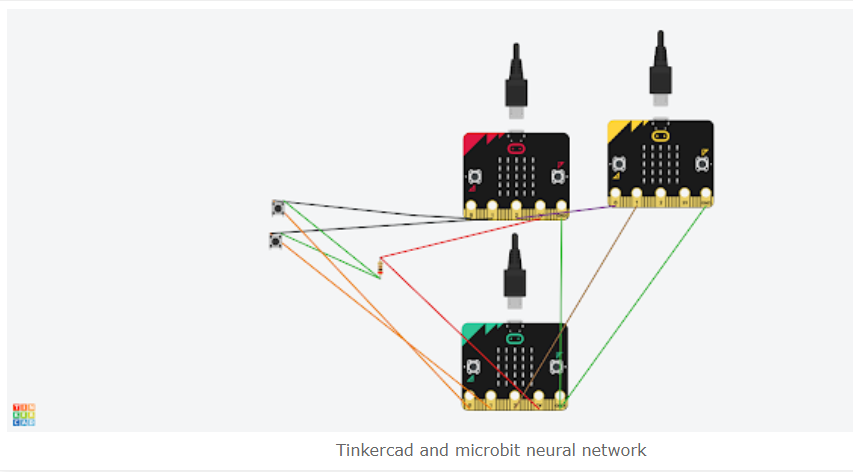
\includegraphics[width=11cm]{chapters/chAi1/figures/Tinkercadann1.png}
    \caption{TinkerCad Microbit Network}
    \label{fig:tinkercad_neural_microbit_network}
\end{figure}
To have a quick play I wonder if using the built in Scratch-like code blocks, I could build a simulation of neuron on the microbit.

Requirements 
- By altering the bias, weights change the behaviour of buttons A and B
-when A is pressed a variable input1 is set to 1 and when released it goes to 0. The same happens for Button B and a variable input 2
- if (bias+weight1*input1+weight2*input2)>=0 then a T for True appears of the LEDs otherwise F for False is shown.
\begin{figure}
    \centering
    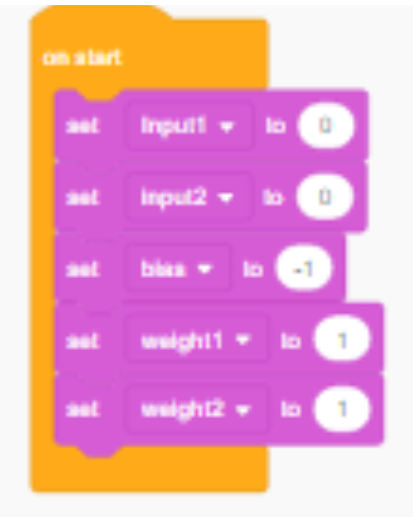
\includegraphics[width=11cm]{chapters/chAi1/figures/Tinkercadann2.png}
    \caption{TinkerCad Microbit Network: setting up}
    \label{fig:tinkercad_neural_microbit_network_basic}
\end{figure}
That is it really, apart initialising the variables. The code for producing an OR is shown below and the GIF at the end shows an AND in action:
\begin{figure}
    \centering
    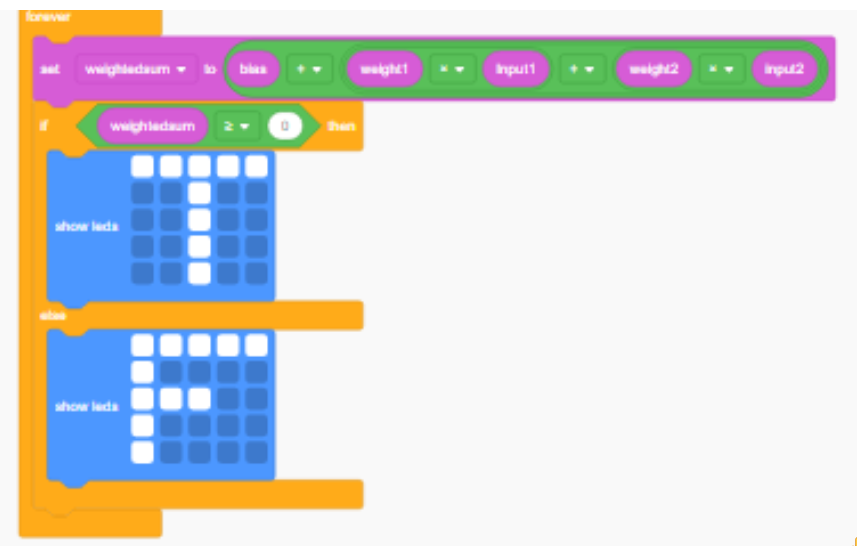
\includegraphics[width=11cm]{chapters/chAi1/figures/Tinkercadann23.png}
    \caption{TinkerCad Microbit Network: basic unit}
    \label{fig:tinkercad_neural_microbit_network_basic2}
\end{figure}
The so in action for an AND (bias is set to -2); change the bias to -1 and you would get an OR.

\begin{figure}
    \centering
    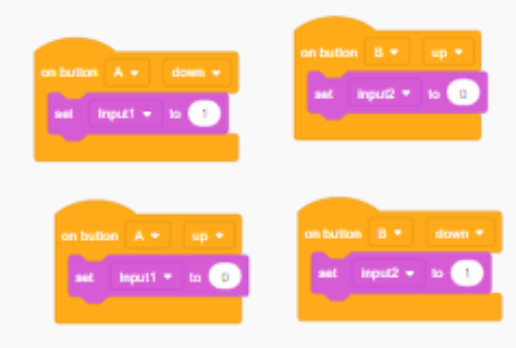
\includegraphics[width=11cm]{chapters/chAi1/figures/Tinkercadann4.png}
    \caption{TinkerCad Microbit Network: }
    \label{fig:tinkercad_neural_microbit_network_basic3}
\end{figure}

The whole thing is available at: \url{https://www.tinkercad.com/things/8Ph6UBFdICz-brave-duup }

Originally published at \url{https://robotsandphysicalcomputing.blogspot.com/2021/01/tinkercad-and-microbit-to-make-neuron.html}


\section{Microbit neural network with TinkerCad}
In a previous post I produced a single neuron based around microbits in Tickercad - see here.

To extend this the basic ideas discussed in that the previous post where extended to three microbit joined together. In  other words a network of neurones or neural network.

Basic requirements of a neuron are
Requirements 
- By altering the bias (or w0 in the example), weights change the behaviour of switches changes.
-when switch is pressed a variable x1 or x2 is set to 1 depending on which button is pressed and when released it goes to 0. 
- if (bias+w1*x1+w2*x2)>=0 then a T for True appears of the LEDs otherwise F for False is shown.

So by selecting the weights and connecting the outputs (p2) from the microbits labelled as Red and Green in the image above as inputs to the yellow microbit 'neuron' we can form a neural network. Switches as the inputs and the screen on the yellow 'neuron' as the output of the network showing true (T) or false(F).

So to build a XOR from the 'neurons'
'hidden layer'
Red microbit had the variables w0 set to -1 and W1 set to 0 and W2 set 1
Green microbit had the variables w0 set to -1 and W1 set to 1 and W2 set 0

'output layer'
Yellow microbit had the variables w0 set to -1 and W1 set to 1 and W2 set 1

All of this can be found at https://www.tinkercad.com/things/hPV4nU0Asr5-smooth-bojo or through the link shown below:

Originally published at \url{https://robotsandphysicalcomputing.blogspot.com/2021/02/making-neural-network-in-tinkercad-from.html}